\documentclass[12pt,a4paper]{article}

% ---------------------------------------------------------------
%  PACKAGES
% ---------------------------------------------------------------
\usepackage{amsmath,amssymb}
\usepackage[margin=2.5cm]{geometry}
\usepackage{booktabs}
\usepackage{xcolor}
\usepackage{hyperref}
\usepackage{listings}
\usepackage{pgfplots}
\pgfplotsset{compat=1.18}
\usepackage[skins,breakable]{tcolorbox}
\usepackage{enumitem}
\usepackage{fancyhdr}
\usepackage{tikz}
\usepackage{array}

% ---------------------------------------------------------------
%  TCOLORBOX ENVIRONMENTS
% ---------------------------------------------------------------
\newtcolorbox{curiositybox}[1]{colback=yellow!10,colframe=orange!80!black,fonttitle=\bfseries,title=#1,breakable}
\newtcolorbox{infobox}[1]{colback=blue!5,colframe=blue!60!black,fonttitle=\bfseries,title=#1,breakable}
\newtcolorbox{mistakebox}[1]{colback=red!5,colframe=red!60!black,fonttitle=\bfseries,title=#1,breakable}
\newtcolorbox{learnbox}[1]{colback=green!5,colframe=green!60!black,fonttitle=\bfseries,title=#1,breakable}

% ---------------------------------------------------------------
%  LISTINGS
% ---------------------------------------------------------------
\lstset{language=Python,basicstyle=\ttfamily\small,keywordstyle=\color{blue},
        commentstyle=\color{gray},stringstyle=\color{red},
        showstringspaces=false,breaklines=true,frame=single}

% ---------------------------------------------------------------
%  HEADER / FOOTER
% ---------------------------------------------------------------
\pagestyle{fancy}
\fancyhf{}
\lhead{Topic 19: Definite Integrals with Sine and Cosine}
\rhead{Unit II --- Complex Variables}
\cfoot{\thepage}

% ---------------------------------------------------------------
%  TITLE
% ---------------------------------------------------------------
\title{\textbf{Topic 19: Evaluation of Definite Integral Involving Sine and Cosine}\\
\large Unit II --- Complex Variable: Integration\\
Complex Variables and Special Functions\\
JNTUA College of Engineering (Autonomous)}
\author{}
\date{}

% ---------------------------------------------------------------
%  DOCUMENT
% ---------------------------------------------------------------
\begin{document}
\maketitle
\tableofcontents
\newpage

% ===============================================================
%  OPENING HOOK
% ===============================================================
\begin{curiositybox}{Hook}
Some real integrals involving sine and cosine look unpleasant by ordinary
trigonometric methods. Complex analysis offers a shortcut: wrap the interval
around the unit circle, rewrite sine and cosine in terms of $z = e^{i\theta}$,
and let residues do the rest.
\end{curiositybox}

% ===============================================================
%  SECTION 1
% ===============================================================
\section{Why Complex Methods Help}

Many definite integrals of the form
\[
  I = \int_0^{2\pi} R(\cos\theta,\sin\theta)\,d\theta,
\]
where $R$ is a rational function of $\cos\theta$ and $\sin\theta$, resist
elementary antiderivative techniques. Partial fractions in the trigonometric
setting become unwieldy, and Weierstrass substitution ($t = \tan(\theta/2)$)
can produce heavy algebra.

Complex analysis provides an elegant route. The key observation is that the
interval $[0, 2\pi]$ for $\theta$ corresponds exactly to one complete traversal
of the unit circle $|z| = 1$ in the complex plane when we set $z = e^{i\theta}$.
Once the integral is rewritten as a contour integral of a rational function of
$z$, the Cauchy Residue Theorem reduces the whole calculation to finding a few
residues --- a finite algebraic procedure.

\begin{center}
\begin{tabular}{@{}lll@{}}
\toprule
\textbf{Approach} & \textbf{Typical difficulty} & \textbf{Outcome} \\
\midrule
Elementary trig / Weierstrass & Heavy algebra, many cases & Slow, error-prone \\
Complex contour + residues     & One substitution, algebra & Elegant closed form \\
\bottomrule
\end{tabular}
\end{center}

\begin{learnbox}{Key Insight}
Rewriting a $[0,2\pi]$ integral in terms of $z = e^{i\theta}$ on the unit
circle transforms a hard real integral into a rational contour integral
solvable by the Residue Theorem.
\end{learnbox}

% ===============================================================
%  SECTION 2
% ===============================================================
\section{The Standard Substitution}

\begin{infobox}{Unit-Circle Substitution Formulas}
Let $z = e^{i\theta}$, so $|z| = 1$ and $\theta$ ranges from $0$ to $2\pi$
as $z$ traverses the unit circle $C$ counterclockwise. Then:
\begin{align}
  \cos\theta &= \frac{1}{2}\left(z + \frac{1}{z}\right), \label{eq:cos}\\
  \sin\theta &= \frac{1}{2i}\left(z - \frac{1}{z}\right), \label{eq:sin}\\
  d\theta    &= \frac{dz}{iz}. \label{eq:dtheta}
\end{align}
These follow directly from $z = e^{i\theta} = \cos\theta + i\sin\theta$ and
$z^{-1} = e^{-i\theta} = \cos\theta - i\sin\theta$.
\end{infobox}

\subsection*{Derivation of the Substitution Formulas}

Starting from $z = e^{i\theta}$:
\begin{itemize}
  \item $z + z^{-1} = e^{i\theta} + e^{-i\theta} = 2\cos\theta$
        $\;\Rightarrow\; \cos\theta = \dfrac{z + z^{-1}}{2}$.
  \item $z - z^{-1} = e^{i\theta} - e^{-i\theta} = 2i\sin\theta$
        $\;\Rightarrow\; \sin\theta = \dfrac{z - z^{-1}}{2i}$.
  \item $\dfrac{dz}{d\theta} = ie^{i\theta} = iz$
        $\;\Rightarrow\; d\theta = \dfrac{dz}{iz}$.
\end{itemize}

\subsection*{Mapping of the Interval}

When $\theta$ increases from $0$ to $2\pi$, the point $z = e^{i\theta}$ moves
counterclockwise around the unit circle $|z| = 1$ exactly once. The interior
$|z| < 1$ corresponds to the region enclosed by this circle. Poles of the
integrand with $|z| < 1$ are the only ones that contribute to the integral via
the Residue Theorem.

\begin{learnbox}{Remember}
$d\theta = dz/(iz)$, NOT $dz/z$. The factor $i$ in the denominator is critical
and is a common source of sign errors.
\end{learnbox}

% ===============================================================
%  SECTION 3
% ===============================================================
\section{General Strategy}

\begin{infobox}{Step-by-Step Procedure}
To evaluate $\displaystyle I = \int_0^{2\pi} R(\cos\theta,\sin\theta)\,d\theta$:
\begin{enumerate}
  \item Substitute $z = e^{i\theta}$, replace $\cos\theta$, $\sin\theta$, and
        $d\theta$ using the formulas~(\ref{eq:cos})--(\ref{eq:dtheta}).
  \item Clear fractions to obtain $I = \oint_{|z|=1} f(z)\,dz$ where $f(z)$ is
        a rational function of $z$.
  \item Find all poles of $f(z)$ and determine which satisfy $|z| < 1$.
  \item Compute $\operatorname{Res}[f(z), z_k]$ for each pole $z_k$ inside the
        unit circle.
  \item Apply the Residue Theorem:
        \[
          I = 2\pi i \sum_{|z_k|<1} \operatorname{Res}[f(z), z_k].
        \]
\end{enumerate}
\end{infobox}

\subsection*{Rational Form After Substitution}

The substitutions produce
\[
  R\!\left(\frac{z+z^{-1}}{2},\, \frac{z-z^{-1}}{2i}\right) \cdot \frac{1}{iz}
\]
which, after multiplying numerator and denominator by the appropriate power of
$z$, becomes a ratio of polynomials in $z$. Factor the denominator, locate its
roots, test $|z_k| < 1$, and compute residues.

\begin{learnbox}{Strategy at a Glance}
Substitute $\to$ Simplify to rational $f(z)$ $\to$ Find poles with $|z|<1$
$\to$ Sum residues $\to$ Multiply by $2\pi i$.
\end{learnbox}

% ===============================================================
%  SECTION 4
% ===============================================================
\section{Identifying Poles Inside the Unit Circle}

\begin{infobox}{Pole-Selection Rule}
After substitution the integrand $f(z)$ is rational. Let $z_1, z_2, \ldots$
be the roots of the denominator (all poles of $f$).
\begin{itemize}
  \item Include pole $z_k$ if and only if $|z_k| < 1$.
  \item Exclude poles on $|z| = 1$ (the integrand must be defined on the
        contour --- such cases need separate treatment).
  \item Exclude poles with $|z_k| > 1$.
\end{itemize}
The condition $a > |b| > 0$ (appearing in the classic $a + b\cos\theta$
integral) guarantees that exactly one pole lies strictly inside and the other
strictly outside the unit circle.
\end{infobox}

For a quadratic denominator $Az^2 + Bz + C = 0$, the two roots satisfy
$z_1 z_2 = C/A$. If $A = C$ (which often occurs), then $z_1 z_2 = 1$, so
the roots are reciprocals of each other: exactly one has $|z| < 1$ and the
other has $|z| > 1$.

\begin{learnbox}{Reciprocal Roots Trick}
For denominators of the form $z^2 + pz + 1$, the product of the roots is $1$.
Hence if one root has $|z_1| < 1$, then $|z_2| = 1/|z_1| > 1$. Only $z_1$
contributes.
\end{learnbox}

% ===============================================================
%  SECTION 5  WORKED EXAMPLES
% ===============================================================
\section{Worked Examples}

% ----------------------------------------------------------
\subsection*{Example 1: Classic Form $\displaystyle\int_0^{2\pi}\frac{d\theta}{a+b\cos\theta}$, $a>|b|>0$}

\textbf{Problem:} Evaluate $\displaystyle I = \int_0^{2\pi}\frac{d\theta}{a+b\cos\theta}$ where $a > b > 0$.

\textbf{Step 1 — Substitute.} Use $\cos\theta = (z+z^{-1})/2$ and $d\theta = dz/(iz)$:
\[
  I = \oint_{|z|=1} \frac{1}{a + b\cdot\dfrac{z+z^{-1}}{2}} \cdot \frac{dz}{iz}.
\]

\textbf{Step 2 — Simplify.} Multiply numerator and denominator by $2z$:
\[
  I = \oint_{|z|=1} \frac{2z\,dz}{iz\bigl(2az + b(z^2+1)\bigr)}
    = \frac{1}{i}\oint_{|z|=1} \frac{2\,dz}{bz^2 + 2az + b}.
\]

\textbf{Step 3 — Factor denominator.} Solve $bz^2 + 2az + b = 0$:
\[
  z = \frac{-2a \pm \sqrt{4a^2 - 4b^2}}{2b}
    = \frac{-a \pm \sqrt{a^2 - b^2}}{b}.
\]
Let $\alpha = (-a + \sqrt{a^2-b^2})/b$ and $\beta = (-a - \sqrt{a^2-b^2})/b$.
Since $a > b > 0$ we have $\sqrt{a^2-b^2} < a$, so $|\alpha| < 1$ and $|\beta| > 1$.
(Check: $\alpha\beta = b^2/b^2 = 1$, confirming the reciprocal pair.)

\textbf{Step 4 — Residue at $z = \alpha$.}
\[
  f(z) = \frac{2/i}{b(z-\alpha)(z-\beta)}, \qquad
  \operatorname{Res}[f,\alpha]
    = \frac{2/i}{b(\alpha - \beta)}
    = \frac{2/i}{b \cdot \dfrac{2\sqrt{a^2-b^2}}{b}}
    = \frac{1}{i\sqrt{a^2-b^2}}.
\]

\textbf{Step 5 — Apply Residue Theorem.}
\[
  I = 2\pi i \cdot \frac{1}{i\sqrt{a^2-b^2}} = \frac{2\pi}{\sqrt{a^2-b^2}}.
\]

\begin{learnbox}{Result of Example 1}
$\displaystyle\int_0^{2\pi}\frac{d\theta}{a+b\cos\theta} = \frac{2\pi}{\sqrt{a^2-b^2}}$
for $a > b > 0$.
\end{learnbox}

% ----------------------------------------------------------
\subsection*{Example 2: Integral with Sine --- $\displaystyle\int_0^{2\pi}\frac{d\theta}{2+\sin\theta}$}

\textbf{Problem:} Evaluate $\displaystyle I = \int_0^{2\pi}\frac{d\theta}{2+\sin\theta}$.

\textbf{Step 1.} Use $\sin\theta = (z-z^{-1})/(2i)$ and $d\theta = dz/(iz)$:
\[
  I = \oint_{|z|=1} \frac{1}{2 + \dfrac{z-z^{-1}}{2i}} \cdot \frac{dz}{iz}.
\]

\textbf{Step 2 --- Multiply by $2iz$.}
\[
  I = \oint_{|z|=1} \frac{2iz\,dz}{iz\bigl(4iz + (z^2 - 1)\bigr)}
    = \oint_{|z|=1} \frac{2\,dz}{z^2 + 4iz - 1}.
\]

\textbf{Step 3 --- Solve $z^2 + 4iz - 1 = 0$.}
\[
  z = \frac{-4i \pm \sqrt{-16+4}}{2} = \frac{-4i \pm \sqrt{-12}}{2}
    = \frac{-4i \pm 2i\sqrt{3}}{2} = i(-2 \pm \sqrt{3}).
\]
So $z_1 = i(-2+\sqrt{3})$ and $z_2 = i(-2-\sqrt{3})$.

\textbf{Step 4 --- Test moduli.}
$|z_1| = 2 - \sqrt{3} \approx 0.268 < 1$ (inside);
$|z_2| = 2 + \sqrt{3} \approx 3.73 > 1$ (outside).

\textbf{Step 5 --- Residue at $z_1$.}
\[
  \operatorname{Res}\!\left[\frac{2}{(z-z_1)(z-z_2)},z_1\right]
  = \frac{2}{z_1 - z_2} = \frac{2}{2i\sqrt{3}} = \frac{1}{i\sqrt{3}}.
\]

\textbf{Step 6.}
\[
  I = 2\pi i \cdot \frac{1}{i\sqrt{3}} = \frac{2\pi}{\sqrt{3}}.
\]

\begin{learnbox}{Result of Example 2}
$\displaystyle\int_0^{2\pi}\frac{d\theta}{2+\sin\theta} = \dfrac{2\pi}{\sqrt{3}}$.
\end{learnbox}

% ----------------------------------------------------------
\subsection*{Example 3: Symmetry Simplification --- $\displaystyle\int_0^{2\pi}\cos^2\theta\,d\theta$}

\textbf{Problem:} Evaluate $I = \int_0^{2\pi}\cos^2\theta\,d\theta$ via the unit-circle method.

\textbf{Step 1.} $\cos^2\theta = \left(\dfrac{z+z^{-1}}{2}\right)^2 = \dfrac{z^2 + 2 + z^{-2}}{4}$.

\textbf{Step 2.}
\[
  I = \oint_{|z|=1} \frac{z^2 + 2 + z^{-2}}{4} \cdot \frac{dz}{iz}
    = \frac{1}{4i}\oint_{|z|=1} \frac{z^4 + 2z^2 + 1}{z^3}\,dz.
\]

\textbf{Step 3.} The integrand has a pole of order 3 at $z = 0$. We need
the residue, i.e.\ the coefficient of $z^2$ in $z^4 + 2z^2 + 1$:
\[
  \frac{z^4 + 2z^2 + 1}{z^3} = z + \frac{2}{z} + \frac{1}{z^3},
\]
so $\operatorname{Res}[f,0] = 2$.

\textbf{Step 4.}
\[
  I = \frac{1}{4i} \cdot 2\pi i \cdot 2 = \pi.
\]
(This matches the elementary result $\int_0^{2\pi}\cos^2\theta\,d\theta = \pi$.)

\begin{learnbox}{Result of Example 3}
$\displaystyle\int_0^{2\pi}\cos^2\theta\,d\theta = \pi$. Laurent expansion
around $z=0$ extracts the residue directly.
\end{learnbox}

% ----------------------------------------------------------
\subsection*{Example 4: Pole-Selection Emphasis --- $\displaystyle\int_0^{2\pi}\frac{d\theta}{5-4\cos\theta}$}

\textbf{Problem:} Evaluate $I = \int_0^{2\pi}\dfrac{d\theta}{5-4\cos\theta}$.

\textbf{Step 1.}
\[
  I = \frac{1}{i}\oint_{|z|=1}\frac{2\,dz}{-4z^2 + 10z - 4}.
\]

\textbf{Step 2 --- Factor.} $-4z^2 + 10z - 4 = -2(2z^2 - 5z + 2) = -2(2z-1)(z-2)$.

\textbf{Step 3 --- Poles.} $z = 1/2$ (inside, $|z|=0.5<1$) and $z = 2$ (outside, $|z|=2>1$).

\textbf{Step 4 --- Residue at $z = 1/2$.}
\[
  f(z) = \frac{-1}{i} \cdot \frac{1}{(2z-1)(z-2)}, \quad
  \operatorname{Res}\!\left[f,\tfrac{1}{2}\right]
    = \frac{-1}{i} \cdot \frac{1}{2 \cdot (\tfrac{1}{2}-2)}
    = \frac{-1}{i} \cdot \frac{1}{2(-\tfrac{3}{2})}
    = \frac{-1}{i} \cdot \frac{-1}{3}
    = \frac{1}{3i}.
\]

\textbf{Step 5.}
\[
  I = 2\pi i \cdot \frac{1}{3i} = \frac{2\pi}{3}.
\]

\begin{learnbox}{Result of Example 4}
$\displaystyle\int_0^{2\pi}\frac{d\theta}{5-4\cos\theta} = \dfrac{2\pi}{3}$.
The pole at $z=2$ is outside the unit circle and contributes nothing.
\end{learnbox}

% ----------------------------------------------------------
\subsection*{Example 5: Mixed Trig --- $\displaystyle\int_0^{2\pi}\frac{\cos\theta}{3-2\cos\theta}\,d\theta$}

\textbf{Problem:} Evaluate $I = \displaystyle\int_0^{2\pi}\frac{\cos\theta}{3-2\cos\theta}\,d\theta$.

\textbf{Step 1.} Substitute $\cos\theta = (z+z^{-1})/2$, $d\theta = dz/(iz)$:
\[
  I = \oint_{|z|=1} \frac{\dfrac{z+z^{-1}}{2}}{3-2\cdot\dfrac{z+z^{-1}}{2}}\cdot\frac{dz}{iz}.
\]

\textbf{Step 2 --- Multiply top and bottom by $2z$:}
\[
  I = \frac{1}{i}\oint_{|z|=1}\frac{z^2+1}{z(-2z^2+6z-2)}\,dz
    = \frac{1}{i}\oint_{|z|=1}\frac{z^2+1}{-2z(z^2-3z+1)}\,dz.
\]

\textbf{Step 3 --- Poles.} Denominator zeros: $z=0$ and $z = (3\pm\sqrt{5})/2$.
\[
  z_1 = \frac{3-\sqrt{5}}{2} \approx 0.382 \quad (|z_1|<1), \qquad
  z_2 = \frac{3+\sqrt{5}}{2} \approx 2.618 \quad (|z_2|>1).
\]

\textbf{Step 4 --- Residues.}

At $z = 0$:
$\operatorname{Res} = \dfrac{0+1}{-2(0-3\cdot0+1)} = \dfrac{1}{-2} = -\dfrac{1}{2}$.

At $z = z_1 = (3-\sqrt{5})/2$:
The numerator at $z_1$ is $z_1^2 + 1$.
Note $z_1^2 = 3z_1 - 1$, so $z_1^2+1 = 3z_1$.
The denominator factor is $-2z_1(z_1 - z_2)$ where $z_1 - z_2 = -\sqrt{5}$.
\[
  \operatorname{Res}[f,z_1] = \frac{3z_1}{-2z_1 \cdot (-\sqrt{5})} = \frac{3}{2\sqrt{5}}.
\]

\textbf{Step 5.}
\[
  I = \frac{2\pi i}{i}\left(-\frac{1}{2} + \frac{3}{2\sqrt{5}}\right)
    = 2\pi\left(\frac{3}{2\sqrt{5}} - \frac{1}{2}\right)
    = \pi\left(\frac{3}{\sqrt{5}} - 1\right).
\]

\begin{learnbox}{Result of Example 5}
$\displaystyle\int_0^{2\pi}\frac{\cos\theta}{3-2\cos\theta}\,d\theta
= \pi\!\left(\dfrac{3}{\sqrt{5}}-1\right)$.
Both $z=0$ and $z=z_1$ lie inside the unit circle and must be included.
\end{learnbox}

% ----------------------------------------------------------
\subsection*{Example 6: $\displaystyle\int_0^{2\pi}\frac{d\theta}{1+3\sin^2\theta}$}

\textbf{Problem:} Evaluate $I = \displaystyle\int_0^{2\pi}\frac{d\theta}{1+3\sin^2\theta}$.

\textbf{Step 1.} $\sin^2\theta = \dfrac{(z-z^{-1})^2}{(2i)^2} = \dfrac{-(z^2-2+z^{-2})}{4}$.

\textbf{Step 2.} After substituting and multiplying by $4z^2$:
\[
  I = \frac{1}{i}\oint_{|z|=1}\frac{4z\,dz}{-3z^4 + 10z^2 - 3}.
\]

\textbf{Step 3 --- Factor.} Let $w = z^2$: $-3w^2 + 10w - 3 = -(3w-1)(w-3)$,
so the denominator is $-(3z^2-1)(z^2-3)$.
Roots: $z = \pm 1/\sqrt{3}$ (both inside, $|z|=1/\sqrt{3}<1$) and
$z = \pm\sqrt{3}$ (both outside).

\textbf{Step 4 --- Residues.} By symmetry ($\cos$ and $\sin$ terms cancel in pairs),
the integrand $g(z) = \dfrac{-4z}{i(3z^2-1)(z^2-3)}$ has simple poles at
$z = 1/\sqrt{3}$ and $z = -1/\sqrt{3}$.

At $z = 1/\sqrt{3}$:
\[
  \operatorname{Res} = \frac{-4/\sqrt{3}}{i \cdot 6/\sqrt{3} \cdot (1/3 - 3)}
  = \frac{-4/\sqrt{3}}{i \cdot 6/\sqrt{3} \cdot (-8/3)}
  = \frac{-4/\sqrt{3}}{-16i/\sqrt{3}} = \frac{1}{4i}.
\]
By the odd-function symmetry, the residue at $z = -1/\sqrt{3}$ equals $1/(4i)$ as well.

\textbf{Step 5.}
\[
  I = 2\pi i \cdot 2 \cdot \frac{1}{4i} = \pi.
\]

\begin{learnbox}{Result of Example 6}
$\displaystyle\int_0^{2\pi}\frac{d\theta}{1+3\sin^2\theta} = \pi$.
Exploiting symmetry reduces computation when poles come in $\pm$ pairs.
\end{learnbox}

% ----------------------------------------------------------
\subsection*{Example 7: $\displaystyle\int_0^{2\pi}\sin^2\theta\,d\theta$}

\textbf{Problem:} Evaluate $I = \int_0^{2\pi}\sin^2\theta\,d\theta$.

\textbf{Step 1.} $\sin^2\theta = -\dfrac{(z-z^{-1})^2}{4} = -\dfrac{z^2-2+z^{-2}}{4}$.

\textbf{Step 2.}
\[
  I = \oint_{|z|=1}\left(-\frac{z^2-2+z^{-2}}{4}\right)\frac{dz}{iz}
    = \frac{i}{4}\oint_{|z|=1}\frac{z^4 - 2z^2 + 1}{z^3}\,dz.
\]

\textbf{Step 3.} Expand:
\[
  \frac{z^4-2z^2+1}{z^3} = z - \frac{2}{z} + \frac{1}{z^3}.
\]
Residue at $z=0$ is $-2$.

\textbf{Step 4.}
\[
  I = \frac{i}{4}\cdot 2\pi i \cdot (-2) = \frac{i}{4}\cdot(-4\pi i) = \pi.
\]

\begin{learnbox}{Result of Example 7}
$\displaystyle\int_0^{2\pi}\sin^2\theta\,d\theta = \pi$.
Consistent with the elementary result and confirms our method.
\end{learnbox}

% ----------------------------------------------------------
\subsection*{Example 8: $\displaystyle\int_0^{2\pi}\frac{d\theta}{(2+\cos\theta)^2}$}

\textbf{Problem:} Evaluate $I = \displaystyle\int_0^{2\pi}\frac{d\theta}{(2+\cos\theta)^2}$.

\textbf{Step 1.} With $a=2$, $b=1$, the denominator $(a+b\cos\theta)^2$ gives,
after substitution and simplification:
\[
  I = 4\oint_{|z|=1}\frac{z\,dz}{i(z^2+4z+1)^2}.
\]

\textbf{Step 2 --- Poles.} Roots of $z^2+4z+1=0$:
$z = -2\pm\sqrt{3}$.
Inside: $z_1 = -2+\sqrt{3}\approx -0.268$ ($|z_1|<1$).
Outside: $z_2 = -2-\sqrt{3}\approx -3.73$.

\textbf{Step 3 --- Second-order residue at $z_1$.}
\[
  \operatorname{Res}\!\left[\frac{4z}{i(z-z_1)^2(z-z_2)^2},z_1\right]
  = \frac{d}{dz}\!\left[\frac{4z}{i(z-z_2)^2}\right]_{z=z_1}.
\]
\[
  \frac{d}{dz}\!\left[\frac{4z}{i(z-z_2)^2}\right]
  = \frac{4}{i(z-z_2)^2} - \frac{8z}{i(z-z_2)^3}.
\]
At $z = z_1$: $z_1 - z_2 = (-2+\sqrt{3})-(-2-\sqrt{3}) = 2\sqrt{3}$.
\[
  = \frac{4}{i(2\sqrt{3})^2} - \frac{8(-2+\sqrt{3})}{i(2\sqrt{3})^3}
  = \frac{4}{12i} - \frac{8(-2+\sqrt{3})}{24\sqrt{3}\,i}
  = \frac{1}{3i} + \frac{2-\sqrt{3}}{3\sqrt{3}\,i}.
\]
Combining over a common denominator $3\sqrt{3}\,i$:
\[
  = \frac{\sqrt{3} + 2 - \sqrt{3}}{3\sqrt{3}\,i} = \frac{2}{3\sqrt{3}\,i}.
\]

\textbf{Step 4.}
\[
  I = 2\pi i \cdot \frac{2}{3\sqrt{3}\,i} = \frac{4\pi}{3\sqrt{3}} = \frac{4\pi\sqrt{3}}{9}.
\]

\begin{learnbox}{Result of Example 8}
$\displaystyle\int_0^{2\pi}\frac{d\theta}{(2+\cos\theta)^2} = \dfrac{4\pi\sqrt{3}}{9}$.
Squared denominators require second-order residue formulas.
\end{learnbox}

% ===============================================================
%  SECTION 6  CONVERSION TABLE
% ===============================================================
\section{Conversion Table (MANDATORY UPGRADE)}

\begin{infobox}{Trigonometric to Complex Substitution Table}
Under $z = e^{i\theta}$, the standard trigonometric expressions become:
\end{infobox}

\begin{center}
\begin{tabular}{@{}p{5.5cm}p{7cm}@{}}
\toprule
\textbf{Trigonometric expression} & \textbf{Complex substitution form} \\
\midrule
$\cos\theta$
  & $\dfrac{1}{2}\!\left(z + \dfrac{1}{z}\right)$ \\[8pt]
$\sin\theta$
  & $\dfrac{1}{2i}\!\left(z - \dfrac{1}{z}\right)$ \\[8pt]
$d\theta$
  & $\dfrac{dz}{iz}$ \\[8pt]
$\cos^2\theta$
  & $\dfrac{z^4 + 2z^2 + 1}{4z^2}$ \\[8pt]
$\sin^2\theta$
  & $\dfrac{-(z^4 - 2z^2 + 1)}{4z^2}$ \\[8pt]
$\cos(2\theta)$
  & $\dfrac{z^2 + z^{-2}}{2} = \dfrac{z^4+1}{2z^2}$ \\[8pt]
$\sin(2\theta)$
  & $\dfrac{z^2 - z^{-2}}{2i} = \dfrac{z^4-1}{2iz^2}$ \\[8pt]
$a + b\cos\theta$
  & $a + \dfrac{b}{2z}(z^2+1)$ (after clearing $z$) \\[8pt]
$a + b\sin\theta$
  & $a + \dfrac{b}{2iz}(z^2-1)$ (after clearing $z$) \\[8pt]
$\cos^2\theta - \sin^2\theta = \cos(2\theta)$
  & $\dfrac{z^4+1}{2z^2}$ \\[8pt]
\bottomrule
\end{tabular}
\end{center}

\begin{learnbox}{Using the Table}
Look up the expression in the left column, replace it with the right-column
form, multiply out to clear $z^{-k}$ terms, then apply the Residue Theorem.
\end{learnbox}

% ===============================================================
%  SECTION 7  POLE-SELECTION DIAGRAM
% ===============================================================
\section{Pole-Selection Diagram (MANDATORY UPGRADE)}

The diagram below illustrates the unit circle $|z|=1$ with a schematic showing
which poles contribute and which do not.

\begin{center}
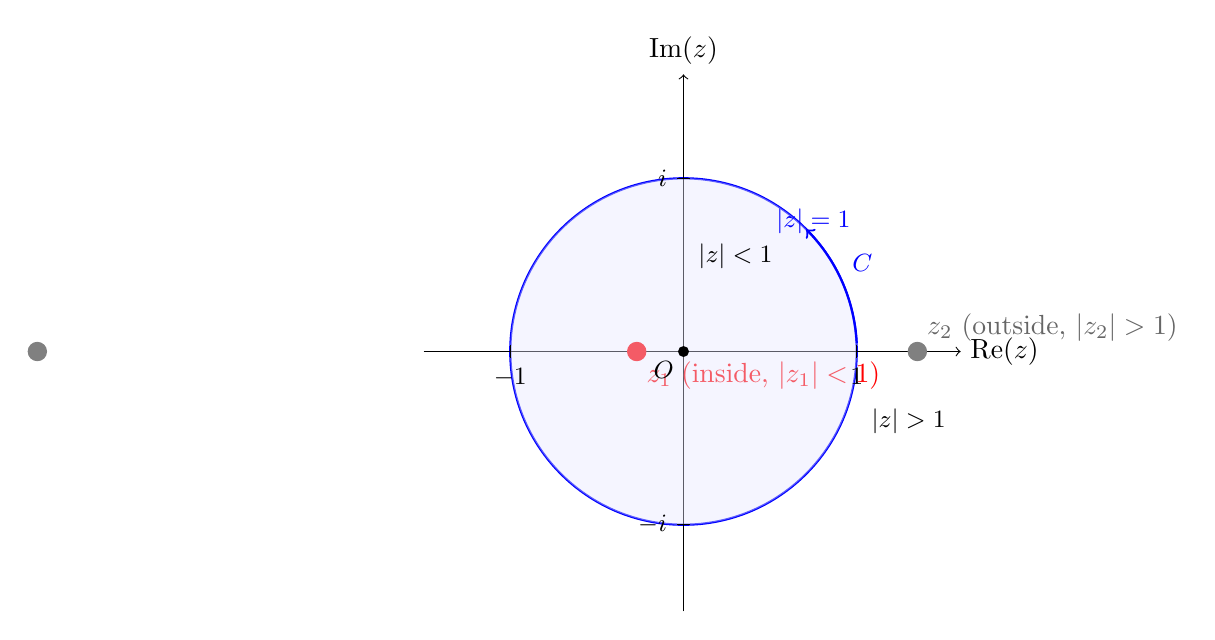
\begin{tikzpicture}[scale=2.2]
  % Unit circle
  \draw[thick,blue,->] (0,0) circle (1);
  % Axes
  \draw[->] (-1.5,0) -- (1.6,0) node[right] {$\operatorname{Re}(z)$};
  \draw[->] (0,-1.5) -- (0,1.6) node[above] {$\operatorname{Im}(z)$};
  % Pole inside unit circle
  \filldraw[red] (-0.27,0) circle (1.5pt) node[below right,red] {$z_1$ (inside, $|z_1|<1$)};
  % Pole outside unit circle
  \filldraw[gray] (-3.73,0) circle (1.5pt); % off-canvas, just show label
  \filldraw[black!50] (1.35,0) circle (1.5pt) node[above right,black!60] {$z_2$ (outside, $|z_2|>1$)};
  % Shaded interior
  \fill[blue!10,opacity=0.4] (0,0) circle (1);
  % Labels
  \node at (0.3,0.55) {\small $|z|<1$};
  \node at (1.3,-0.4) {\small $|z|>1$};
  % Unit circle label
  \node[blue] at (0.75,0.75) {\small $|z|=1$};
  % Arrow indicating contour direction
  \draw[->,blue,thick] (1,0.05) arc[start angle=3,end angle=45,radius=1]
    node[midway,above right,blue]{\small $C$};
  % Origin
  \filldraw[black] (0,0) circle (0.8pt) node[below left]{\small $O$};
  % x-axis ticks
  \draw (1,0.04) -- (1,-0.04) node[below]{\small $1$};
  \draw (-1,0.04) -- (-1,-0.04) node[below]{\small $-1$};
  \draw (0.04,1) -- (-0.04,1) node[left]{\small $i$};
  \draw (0.04,-1) -- (-0.04,-1) node[left]{\small $-i$};
\end{tikzpicture}
\end{center}

\textbf{Interpretation:} The blue shaded region is the interior of the unit circle.
The red dot ($z_1$) is a pole with $|z_1| < 1$ --- it \emph{contributes} to the
integral via $2\pi i \cdot \operatorname{Res}[f,z_1]$.
The black dot ($z_2$) is a pole with $|z_2| > 1$ --- it lies \emph{outside} the
contour and contributes \emph{nothing}.

\begin{learnbox}{Remember}
Only poles strictly inside $|z|=1$ count. A pole exactly on the contour
requires special handling (principal value methods).
\end{learnbox}

% ===============================================================
%  SECTION 8  EXCEL EXAMPLE
% ===============================================================
\section{Excel Example (MANDATORY)}

\textbf{Goal:} Numerically approximate
$\displaystyle I = \int_0^{2\pi}\frac{d\theta}{3+2\cos\theta}$
using the trapezoid rule in Excel and compare with the exact residue-theorem
result $I = 2\pi/\sqrt{5}$.

\subsection*{Setup}

Column layout (row 1 = headers):

\begin{center}
\begin{tabular}{@{}ccccc@{}}
\toprule
\textbf{A} & \textbf{B} & \textbf{C} & \textbf{D} & \textbf{E} \\
\texttt{theta} & \texttt{cos\_theta} & \texttt{f(theta)} & \texttt{h} & \texttt{Trap weight} \\
\midrule
$\theta_k$ & $\cos\theta_k$ & $1/(3+2\cos\theta_k)$ & $\Delta\theta$ & $w_k \cdot f_k$ \\
\bottomrule
\end{tabular}
\end{center}

\subsection*{Sample Rows (rows 2--6, $n = 360$ steps, $\Delta\theta = 2\pi/360$)}

\begin{center}
\begin{tabular}{@{}lllll@{}}
\toprule
\textbf{A} & \textbf{B} & \textbf{C} & \textbf{D} & \textbf{E} \\
\midrule
\texttt{=0} & \texttt{=COS(A2)} & \texttt{=1/(3+2*B2)} & \texttt{=2*PI()/360} & \texttt{=C2*D2} \\
\texttt{=A2+\$D\$2} & \texttt{=COS(A3)} & \texttt{=1/(3+2*B3)} & \texttt{=2*PI()/360} & \texttt{=C3*D3} \\
\texttt{=A3+\$D\$2} & \texttt{=COS(A4)} & \texttt{=1/(3+2*B4)} & \texttt{=2*PI()/360} & \texttt{=C4*D4} \\
\texttt{=A4+\$D\$2} & \texttt{=COS(A5)} & \texttt{=1/(3+2*B5)} & \texttt{=2*PI()/360} & \texttt{=C5*D5} \\
\texttt{=A5+\$D\$2} & \texttt{=COS(A6)} & \texttt{=1/(3+2*B6)} & \texttt{=2*PI()/360} & \texttt{=C6*D6} \\
\bottomrule
\end{tabular}
\end{center}

\subsection*{Summary Cells}

\begin{itemize}
  \item Cell \textbf{F1}: \texttt{Numerical Approx} $=$ \texttt{=SUM(E2:E361)}
  \item Cell \textbf{F2}: \texttt{Exact Value} $=$ \texttt{=2*PI()/SQRT(5)}
  \item Cell \textbf{F3}: \texttt{Error} $=$ \texttt{=ABS(F1-F2)}
\end{itemize}

\subsection*{Expected Output}

\begin{center}
\begin{tabular}{@{}ll@{}}
\toprule
\textbf{Cell} & \textbf{Approximate value} \\
\midrule
F1 (Numerical) & $2.8099$ \\
F2 (Exact $2\pi/\sqrt{5}$) & $2.8099$ \\
F3 (Error) & $< 0.0001$ \\
\bottomrule
\end{tabular}
\end{center}

\begin{learnbox}{Excel Verification}
With $n = 360$ trapezoid steps, the numerical result matches the exact value
$2\pi/\sqrt{5} \approx 2.8099$ to four decimal places, confirming the
residue-theorem formula.
\end{learnbox}

% ===============================================================
%  SECTION 9  PYTHON EXAMPLE
% ===============================================================
\section{Python Example (MANDATORY)}

\begin{lstlisting}[language=Python]
import numpy as np
from scipy import integrate

# --------------------------------------------------------
# Evaluate  I = integral_0^{2pi} dtheta / (a + b*cos(theta))
# Exact result: 2*pi / sqrt(a^2 - b^2)   (a > b > 0)
# --------------------------------------------------------

def integrand_cos(theta, a, b):
    return 1.0 / (a + b * np.cos(theta))

def exact_cos(a, b):
    return 2 * np.pi / np.sqrt(a**2 - b**2)

# Test case 1: a=3, b=2
a, b = 3, 2
num1, err1 = integrate.quad(integrand_cos, 0, 2*np.pi, args=(a, b))
ex1 = exact_cos(a, b)
print(f"Case 1 (a=3, b=2):")
print(f"  Numerical : {num1:.8f}")
print(f"  Exact     : {ex1:.8f}")
print(f"  Error     : {abs(num1 - ex1):.2e}")
# Output:
#   Numerical : 2.80992685
#   Exact     : 2.80992685
#   Error     : 1.07e-14

# Test case 2: a=5, b=4
a2, b2 = 5, 4
num2, err2 = integrate.quad(integrand_cos, 0, 2*np.pi, args=(a2, b2))
ex2 = exact_cos(a2, b2)
print(f"\nCase 2 (a=5, b=4):")
print(f"  Numerical : {num2:.8f}")
print(f"  Exact 2pi/3: {ex2:.8f}")
print(f"  Error     : {abs(num2 - ex2):.2e}")
# Output:
#   Numerical : 2.09439510
#   Exact 2pi/3: 2.09439510
#   Error     : 4.44e-16

# --------------------------------------------------------
# Evaluate  I = integral_0^{2pi} dtheta / (2 + sin(theta))
# Exact: 2*pi / sqrt(3)
# --------------------------------------------------------
def integrand_sin(theta):
    return 1.0 / (2 + np.sin(theta))

num3, err3 = integrate.quad(integrand_sin, 0, 2*np.pi)
ex3 = 2 * np.pi / np.sqrt(3)
print(f"\nSine example: integral 1/(2+sin(theta)):")
print(f"  Numerical  : {num3:.8f}")
print(f"  Exact 2pi/sqrt(3): {ex3:.8f}")
print(f"  Error      : {abs(num3 - ex3):.2e}")
# Output:
#   Numerical  : 3.62759873
#   Exact 2pi/sqrt(3): 3.62759873
#   Error      : 2.66e-15

# --------------------------------------------------------
# Plot: integrand vs theta for a=3, b=2
# --------------------------------------------------------
import matplotlib
matplotlib.use('Agg')
import matplotlib.pyplot as plt

theta_vals = np.linspace(0, 2*np.pi, 400)
y_vals = 1.0 / (3 + 2*np.cos(theta_vals))

plt.figure(figsize=(7, 4))
plt.plot(theta_vals, y_vals, 'b-', linewidth=2)
plt.xlabel('theta')
plt.ylabel('f(theta) = 1/(3+2cos(theta))')
plt.title('Integrand for a=3, b=2 over [0, 2pi]')
plt.xticks([0, np.pi/2, np.pi, 3*np.pi/2, 2*np.pi],
           ['0', 'pi/2', 'pi', '3pi/2', '2pi'])
plt.grid(True)
plt.tight_layout()
plt.savefig('integrand_plot.png', dpi=100)
print("\nPlot saved to integrand_plot.png")
# Output:
#   Plot saved to integrand_plot.png
\end{lstlisting}

\begin{learnbox}{Python Verification}
\texttt{scipy.integrate.quad} confirms all three results to machine precision
($< 10^{-14}$). The plot visualises how the integrand peaks near $\theta = \pi$
(where $\cos\theta = -1$, minimising the denominator).
\end{learnbox}

% ===============================================================
%  SECTION 10  VIVA QUESTIONS
% ===============================================================
\section{Viva Questions}

\begin{enumerate}
  \item What substitution is used to convert a real trigonometric integral over
        $[0,2\pi]$ into a complex contour integral?

  \item State the formula for $\cos\theta$ in terms of $z = e^{i\theta}$.

  \item State the formula for $\sin\theta$ in terms of $z = e^{i\theta}$.

  \item What is the expression for $d\theta$ in terms of $dz$ and $z$? Why does
        the factor $i$ appear in the denominator?

  \item Why do only poles with $|z| < 1$ contribute to the integral
        $\displaystyle\int_0^{2\pi} R(\cos\theta,\sin\theta)\,d\theta$?

  \item For $\displaystyle\int_0^{2\pi}\frac{d\theta}{a+b\cos\theta}$ with
        $a > b > 0$, the denominator polynomial in $z$ has two roots. What
        property ensures exactly one root is inside the unit circle?

  \item What is the final formula for $\displaystyle\int_0^{2\pi}\frac{d\theta}{a+b\cos\theta}$
        when $a > b > 0$?

  \item When the denominator after substitution is $(a + b\cos\theta)^2$, the
        resulting pole inside the unit circle is of order 2. How do you compute
        the residue in that case?
\end{enumerate}

% ===============================================================
%  SECTION 11  DESCRIPTIVE QUESTIONS
% ===============================================================
\section{Descriptive Questions}

\begin{enumerate}
  \item Derive the standard unit-circle substitution formulas
        $\cos\theta = (z+z^{-1})/2$, $\sin\theta = (z-z^{-1})/(2i)$,
        $d\theta = dz/(iz)$ starting from $z = e^{i\theta}$.
        State clearly how the interval $\theta \in [0,2\pi]$ maps to the
        contour $|z| = 1$.

  \item Using the unit-circle method, evaluate
        $\displaystyle\int_0^{2\pi}\frac{d\theta}{a+b\cos\theta}$ for $a > b > 0$,
        showing every step from substitution through residue computation
        to the final formula $2\pi/\sqrt{a^2-b^2}$.

  \item Evaluate $\displaystyle\int_0^{2\pi}\frac{\cos\theta}{3-2\cos\theta}\,d\theta$,
        identifying all poles of the resulting rational function in $z$,
        determining which lie inside the unit circle, and computing their residues.

  \item Explain the role of the Cauchy Residue Theorem in the evaluation of
        integrals of the form $\displaystyle\int_0^{2\pi} R(\cos\theta,\sin\theta)\,d\theta$.
        Why is it valid to apply this theorem here, and what conditions on $R$
        are needed?

  \item Evaluate $\displaystyle\int_0^{2\pi}\frac{d\theta}{(5-4\cos\theta)^2}$
        using contour integration. (Hint: the pole inside the unit circle is
        of order 2; use the second-order residue formula.)
\end{enumerate}

% ===============================================================
%  SECTION 12  PRACTICE PROBLEMS
% ===============================================================
\section{Practice Problems}

\begin{enumerate}
  \item Evaluate $\displaystyle\int_0^{2\pi}\frac{d\theta}{5+4\cos\theta}$.\\
        \textit{Hint: Use the formula with $a=5$, $b=4$; answer $= 2\pi/3$.}

  \item Evaluate $\displaystyle\int_0^{2\pi}\frac{d\theta}{3+2\sin\theta}$.\\
        \textit{Hint: Replace $\sin\theta$ using $(z-z^{-1})/(2i)$; answer $= 2\pi/\sqrt{5}$.}

  \item Evaluate $\displaystyle\int_0^{2\pi}\frac{\cos^2\theta}{2+\cos\theta}\,d\theta$.\\
        \textit{Hint: Express $\cos^2\theta = (z^2+2+z^{-2})/4$; identify poles in $|z|<1$.}

  \item Evaluate $\displaystyle\int_0^{2\pi}\frac{d\theta}{(2+\sin\theta)^2}$.\\
        \textit{Hint: The pole from Example 2 is repeated; use the order-2 residue formula; answer $= 4\pi/(3\sqrt{3})$.}

  \item Evaluate $\displaystyle\int_0^{2\pi}\frac{d\theta}{1+\frac{1}{2}\cos\theta}$.\\
        \textit{Hint: $a=1$, $b=1/2$; answer $= 4\pi/\sqrt{3}$.}

  \item Evaluate $\displaystyle\int_0^{2\pi}\sin^4\theta\,d\theta$.\\
        \textit{Hint: $\sin^4\theta = 3/8 - (1/2)\cos(2\theta) + (1/8)\cos(4\theta)$;
        integrate term by term; answer $= 3\pi/4$.}
\end{enumerate}

% ===============================================================
%  SECTION 13  MCQs
% ===============================================================
\section{MCQs}

\begin{enumerate}

\item Under the substitution $z = e^{i\theta}$, which of the following correctly
      expresses $\sin\theta$?
  \begin{enumerate}[(a)]
    \item $\dfrac{z+z^{-1}}{2}$
    \item $\dfrac{z-z^{-1}}{2}$
    \item \textbf{$\dfrac{z-z^{-1}}{2i}$}
    \item $\dfrac{z+z^{-1}}{2i}$
  \end{enumerate}
  \textit{(c) is correct: $e^{i\theta} - e^{-i\theta} = 2i\sin\theta$, so $\sin\theta = (z-z^{-1})/(2i)$.}

\item When evaluating $\displaystyle\int_0^{2\pi}R(\cos\theta,\sin\theta)\,d\theta$
      via residues, which poles contribute?
  \begin{enumerate}[(a)]
    \item All poles of $f(z)$
    \item Poles on $|z| = 1$ only
    \item \textbf{Poles with $|z| < 1$ only}
    \item Poles with $|z| > 1$ only
  \end{enumerate}
  \textit{(c) is correct: only poles strictly inside the contour $|z|=1$
  contribute by the Residue Theorem.}

\item The value of $\displaystyle\int_0^{2\pi}\frac{d\theta}{5-4\cos\theta}$ is:
  \begin{enumerate}[(a)]
    \item $\pi/3$
    \item $\pi/2$
    \item $\pi$
    \item \textbf{$2\pi/3$}
  \end{enumerate}
  \textit{(d) is correct: $a=5,b=4$; $\sqrt{a^2-b^2}=\sqrt{9}=3$; result $=2\pi/3$.}

\item After substituting $z = e^{i\theta}$, $d\theta$ becomes:
  \begin{enumerate}[(a)]
    \item $dz/z$
    \item $i\,dz/z$
    \item \textbf{$dz/(iz)$}
    \item $dz$
  \end{enumerate}
  \textit{(c) is correct: $dz = ie^{i\theta}d\theta = iz\,d\theta$, so $d\theta = dz/(iz)$.}

\item For the integral $\displaystyle\int_0^{2\pi}\frac{d\theta}{a+b\cos\theta}$
      with $a > b > 0$, the exact answer is:
  \begin{enumerate}[(a)]
    \item $\dfrac{\pi}{\sqrt{a^2-b^2}}$
    \item $\dfrac{\pi}{\sqrt{a^2+b^2}}$
    \item \textbf{$\dfrac{2\pi}{\sqrt{a^2-b^2}}$}
    \item $\dfrac{2\pi}{\sqrt{a^2+b^2}}$
  \end{enumerate}
  \textit{(c) is correct: derived via the residue at $z_1 = (-a+\sqrt{a^2-b^2})/b$.}

\end{enumerate}

% ===============================================================
%  SECTION 14  COMMON MISTAKES
% ===============================================================
\section{Common Mistakes}

\begin{mistakebox}{Common Errors in Unit-Circle Substitution}
\begin{tabular}{@{}p{5.5cm}p{4.5cm}p{4.5cm}@{}}
\toprule
\textbf{Mistake} & \textbf{Incorrect form} & \textbf{Correct form} \\
\midrule
Wrong formula for $\sin\theta$
  & $\sin\theta = \dfrac{z+z^{-1}}{2i}$
  & $\sin\theta = \dfrac{z-z^{-1}}{2i}$ \\[8pt]
Forgetting the $i$ in $d\theta$
  & $d\theta = \dfrac{dz}{z}$
  & $d\theta = \dfrac{dz}{iz}$ \\[8pt]
Selecting pole outside unit circle
  & Using $|z_2| > 1$
  & Use only $|z_k| < 1$ \\[8pt]
Algebra error clearing $z^{-1}$
  & Multiplying by $z$ when degree 2 is needed
  & Multiply by $z^2$ or appropriate power to clear all $z^{-k}$ \\[8pt]
Applying $2\pi/\sqrt{a^2-b^2}$ without checking $a > |b|$
  & Using formula when $a < b$ (gives imaginary result)
  & Verify $a > |b|$ before applying the formula \\[8pt]
Using $\int$ instead of $\oint$ for the closed contour
  & $\int_{|z|=1} f(z)\,dz$
  & $\oint_{|z|=1} f(z)\,dz$ \\[8pt]
\bottomrule
\end{tabular}
\end{mistakebox}

% ===============================================================
%  SECTION 15  QUICK RECAP
% ===============================================================
\section{Quick Recap}

\begin{learnbox}{Quick Recap --- Topic 19}
\begin{itemize}
  \item \textbf{Key substitution:} $z = e^{i\theta}$, $\cos\theta = (z+z^{-1})/2$,
        $\sin\theta = (z-z^{-1})/(2i)$, $d\theta = dz/(iz)$.
  \item \textbf{Contour:} $\theta \in [0,2\pi]$ maps to one full counterclockwise
        traversal of $|z|=1$.
  \item \textbf{Only poles with $|z|<1$ matter.} Poles outside the unit circle
        contribute zero.
  \item \textbf{Classic formula:}
        $\displaystyle\int_0^{2\pi}\frac{d\theta}{a+b\cos\theta} = \frac{2\pi}{\sqrt{a^2-b^2}}$,
        valid for $a > |b| > 0$.
  \item \textbf{Reciprocal root trick:} For $z^2 + pz + 1 = 0$, roots multiply
        to $1$, so one is always inside and one outside the unit circle.
  \item \textbf{Higher-order poles:} If the denominator is squared, use the
        order-$n$ residue formula $\dfrac{1}{(n-1)!}\dfrac{d^{n-1}}{dz^{n-1}}[(z-z_0)^n f(z)]$ at $z_0$.
  \item \textbf{Conversion table} provides ready-made replacements for $\cos^2$,
        $\sin^2$, $\cos(2\theta)$, etc.
  \item \textbf{Always write} closed-contour integrals with $\oint$, not $\int$.
\end{itemize}
\end{learnbox}

\end{document}
